% -*- root: rapport.tex -*-
\documentclass[a4paper, 12pt]{article}
\usepackage{graphicx}
\DeclareGraphicsExtensions{.pdf,.png,.jpg}
\usepackage{xcolor}   %May be necessary if you want to color links
\usepackage{hyperref}
\usepackage{mathtools}
\usepackage{listings}
\usepackage{pgfplots}
\usepackage{pgfplotstable}
\usepackage{booktabs}
%\usepackage{inconsolata}




\hypersetup{
    colorlinks=true, %set true if you want colored links
    linktoc=all,     %set to all if you want both sections and subsections linked
    citecolor=black,
    filecolor=black,
    linkcolor=black,
    urlcolor=blue
}

\lstdefinestyle{customc}{
  belowcaptionskip=1\baselineskip,
  breaklines=true,
  frame=single,
  language=C,
  showstringspaces=false,
  basicstyle=\footnotesize\ttfamily,
  keywordstyle=\bfseries\color{green!40!black},
  commentstyle=\itshape\color{purple!40!black},
  identifierstyle=\color{blue},
  stringstyle=\color{orange},
  tabsize=4
}
\lstset{escapechar=@,style=customc}

\title{Utilizing Amazon's Zookeeper to handle scaling and maintenance of a Voldemort cluster}
\author{Eivind Siqveland Larsen and Knut Nygaard,\\
        Department of Computer Science,\\
        NTNU,
        Trondheim}

\begin{document}
\maketitle
\thispagestyle{empty}

\clearpage

\begin{abstract}
NoSQL databases often support scalability and high availability.
We address Voldemort, which is a popular, highly available NoSQL database that can be run on several nodes.
The system is cumbersome to setup and maintain. As clusters grow in size, scaling into hundreds of nodes, management and administrative tasks become increasingly complex. We have therefore focused on automating management of a running cluster of nodes.

We have migrated the configuration storage of the Voldemort distributed NoSQL database from local XML files on disk to global objects using Apache ZooKeeper.

Using native tools and ZooKeeper coordination, we have implemented a fault tolerant, redundant service. The service manages node discovery, configuration generation and propagation. It also has components for live monitoring and adjustment of responsibility to match each nodes available system resources.

\end{abstract}

\clearpage
\renewcommand{\abstractname}{Sammendrag}
\begin{abstract}
Vi har flyttet konfigurasjon av en distribuert NoSql database fra lokalt lagrede XML filer til globalt tilgjengelige objekter ved hjelp av Apache ZooKeeper.

Vi har brukt ZooKeepers egenskaper for koordinasjon og andre verktøy til å implementere en feiltolerant, redundant tjeneste for å ta hånd om nye noder, generere konfigurasjonsfiler, propagere endringer og automatisk tilpassing av det kjørende systemet til den enkelte nodes tilgjengelige systemressurser.
\end{abstract}

\setcounter{page}{1}

\clearpage
\tableofcontents

\clearpage
\listoffigures

\clearpage

\section{Hardware}
\label{sec:hardware}

\subsection{Mac Mini}
We server running voldemort is a a Mac Mini Mid 2010 model. It has a Intel Core Duo 2.4 GHz processor, 8 GBs of RAM and solid state storage. We run the latest OS X 10.9.1

\begin{figure}[h]
    \centering
    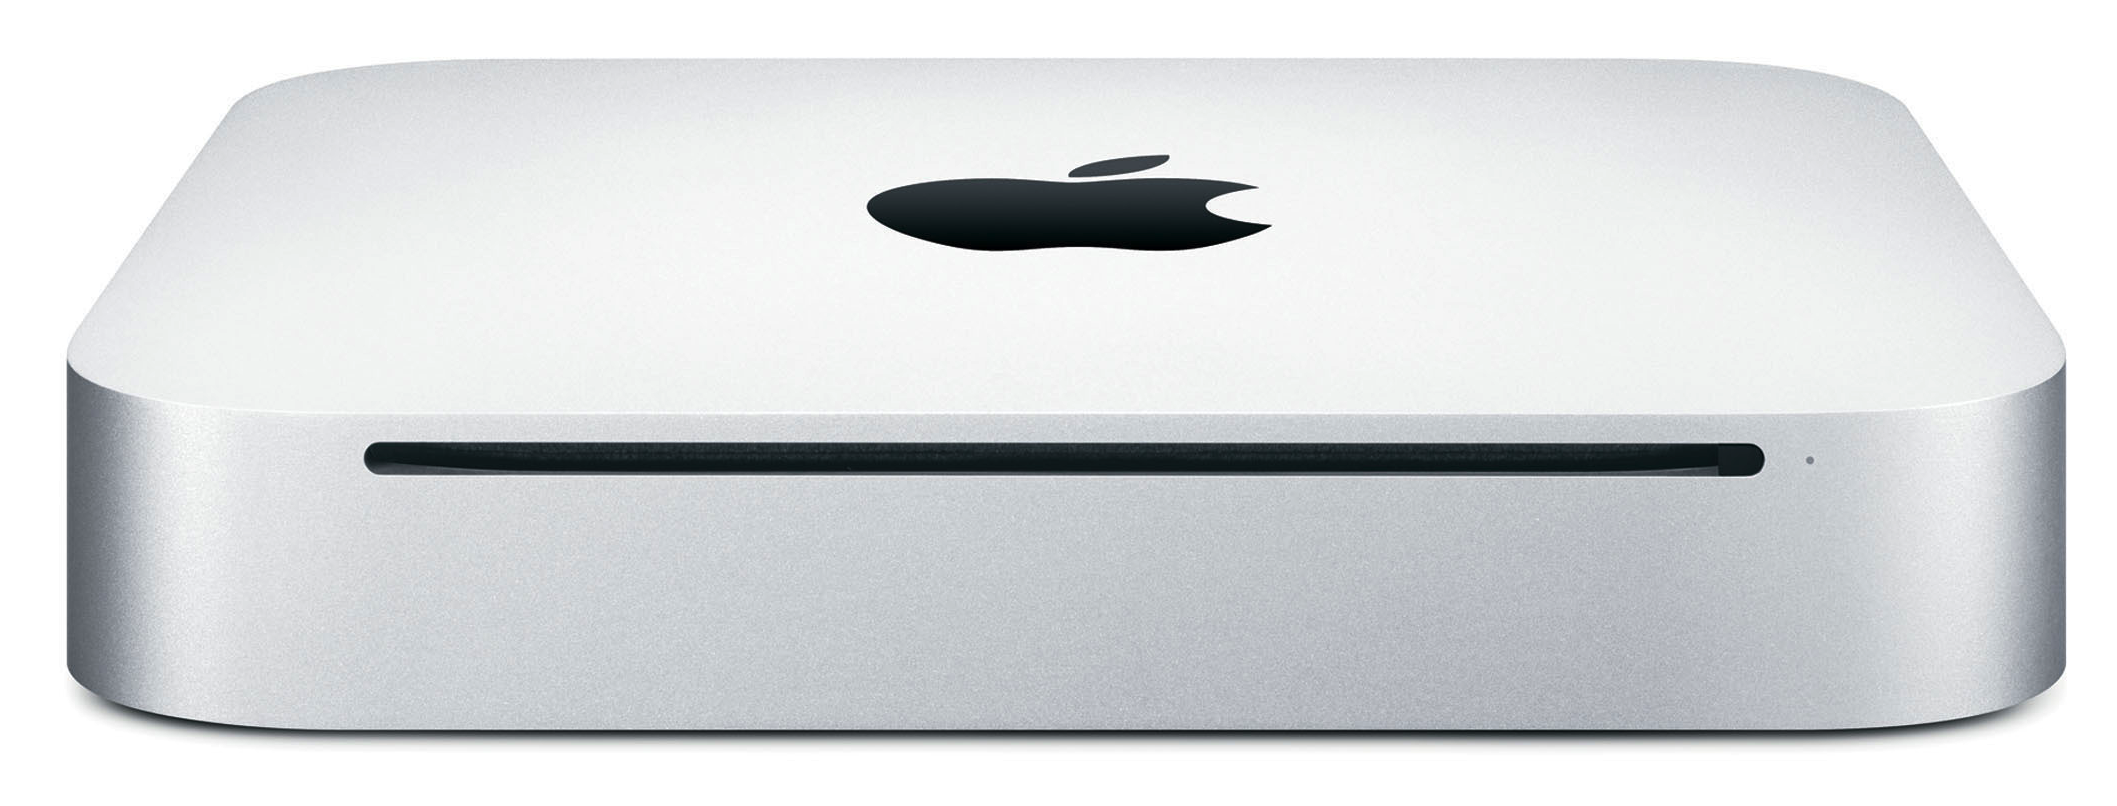
\includegraphics[width=0.8\textwidth]{hardware/mac-mini-06-2010}
    \caption{Mac Mini 2010}
    \label{fig:macmini_hw}
\end{figure}



\clearpage
\bibliographystyle{plain}
\bibliography{references}

\end{document}
